\documentclass[12pt]{article}
\usepackage[T1]{fontenc}
\usepackage[utf8]{inputenc}
\usepackage{url}
\usepackage{enumerate}
\usepackage[top=3cm, bottom=3cm]{geometry}
\usepackage{graphicx} 
\usepackage{enumitem}
\usepackage{natbib}
\usepackage{listings}
\usepackage{float}
\usepackage{amsmath}
\usepackage{color}
\bibpunct{[}{]}{,}{a}{}{;}
\setcitestyle{super}

% Variables
\newcommand{\assignmentname}{Assignment 2}
\newcommand{\coursename}{Statistical Methods in Machine Learning}
\newcommand{\studentnameOne}{Bjarki Madsen (lch929)}
\newcommand{\studentnameTwo}{Disha Singh (cfn492)}
\newcommand{\studentnameThree}{Sokratis Siozos - Drosos (dnb823)}
\newcommand{\department}{Department of Computer Science}
\newcommand{\institution}{Copenhagen University}
\newcommand{\location}{Copenhagen, Denmark}

\begin{document}

\renewcommand\refname{References}

\title{\assignmentname \\ {\Large {\textsc \coursename}}}
\author{
        \studentnameOne \\
        \studentnameTwo \\
        \studentnameThree \\ \\
                \department \\
        \institution \\
        \location
}
\date{5/3/2015}

\maketitle
\thispagestyle{empty}

\pagebreak

\section*{II.1 Classification}

  \subsection*{II.1.1 Linear discriminant analysis}

    The implementation for LDA is found in the function \texttt{LDA} in \texttt{assignment2.py}. The reported accuracies of the classifier are shown in Table \ref{table:accuracy_LDA}.

    \begin{table}[h]
      \centering
      \begin{tabular}{lllll}
        \cline{2-3}
        \multicolumn{1}{l|}{}                & \multicolumn{1}{l|}{Training} & \multicolumn{1}{l|}{Test}  &  &  \\ \cline{1-3}
        \multicolumn{1}{|l|}{Non-normalized} & \multicolumn{1}{l|}{0.860}    & \multicolumn{1}{l|}{0.816} &  &  \\
        \multicolumn{1}{|l|}{Normalized}     & \multicolumn{1}{l|}{0.860}    & \multicolumn{1}{l|}{0.816} &  &  \\ \cline{1-3}
        \end{tabular}
      \caption{Accuracy for the LDA classifier for both non- and normalized data. }
      \label{table:accuracy_LDA}
    \end{table}

  \subsection*{II.1.2 LDA and normalization} 

    The accuracy of the LDA classifier on the normalized data is shown in Table \ref{table:accuracy_LDA}. The result is the same as LDA learns from the covariance matrix. Being a linear transformation of the covariance matrix. It remains same as covariance matrix and its inverse together doesn't effect its lear transformation so it does not effect LDA and remains the same. 

  \subsection*{II.1.3 Bayes optimal classification and probabilistic classification}

    The optimal classification is found with:
      $$ argmax_k Pr(Y = C_k | X = x) $$ 
    Trying $k = 0$:
      \begin{align*}
        Pr(Y=0|X=0) &= \frac{p(X=0|Y=0) \times Pr(Y=0)}{p(X=0)} \\
                    &= \frac{1 * 1/4}{1} = \frac{1}{4}
      \end{align*}
    and $k = 1$:
      \begin{align*}
        Pr(Y=1|X=0) &= \frac{p(X=0|Y=1) \times Pr(Y=1)}{p(X=0)} \\
                    &= \frac{1 * 3/4}{1} = \frac{3}{4}
      \end{align*}
    and therefore the optimal classification is given by $k=1$ where the risk is 0.25 since the optimal classification would only be correct in 3 out of 4, given the output $S$.\\
    
    Considering the probabilistic classifier that predicts 0 with a probability of 0.25 and 1 with 0.75. Since we already computed probability of getting a zero given zero and probability of getting one given a zero. The actual risk of probabilistic classifier can be given as:\\
    \begin{align*}
      R(W) &= p(Y=0/X=0) * p(Y = 1) + p(Y = 1/ X= 0) * p(Y = 0) \\ 
      R(W) &= 0.25 * 0.75 + 0.75 * 0.25\\
      R(W) &= 0.1875 + 0.1875\\
      R(W) &= 0.3750
    \end{align*}
Risk of probabilistic classifier, that is loss is given by 0.375




\section*{II.2 Regression: Sunspot Prediction}

  \subsection*{II.2.1 Maximum likelihood solution}

    The code for this section is found in \texttt{ii\_2\_1(), ML\_regression()} and \texttt{RMSE()}. The reported root mean square error (RMS) for each model used on the test data is shown in table \ref{table:rms_errors}. As the table shows, the error is the lowest for selection 3, which does not come as a surprise since that model includes all the columns of the training data. In figure \ref{fig:years_vs_predicted} it is also possible to see how well the selection 3 model fits the actual model better than the other two models.

    \begin{table}[h]
      \centering
      \begin{tabular}{l|l|lll}
      \cline{2-2}
                                              & RMS error &  &  &  \\ \cline{1-2}
      \multicolumn{1}{|l|}{Selection 1 model} & 35.47     &  &  &  \\
      \multicolumn{1}{|l|}{Selection 2 model} & 28.84     &  &  &  \\
      \multicolumn{1}{|l|}{Selection 3 model} & 18.77     &  &  &  \\ \cline{1-2}
      \end{tabular}
      \caption{RMS errors using ML models for selection 1-3.}
      \label{table:rms_errors}
    \end{table}

    \begin{figure}[h]
      \centering
        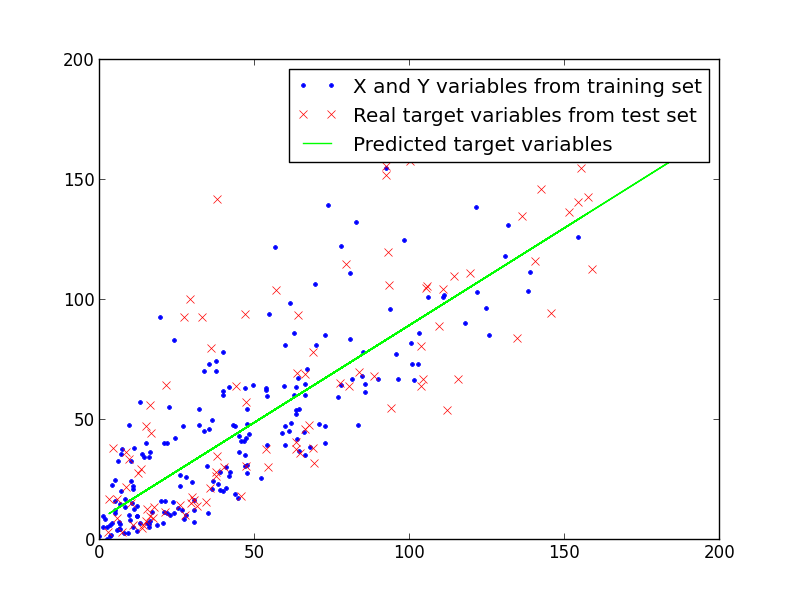
\includegraphics[width=1.0\textwidth]{figures/figure_II_2_1_1}
      \caption{Predicted target variables upon training and data set.}
      \label{fig:target_vars}
    \end{figure}

    \begin{figure}[h]
      \centering
        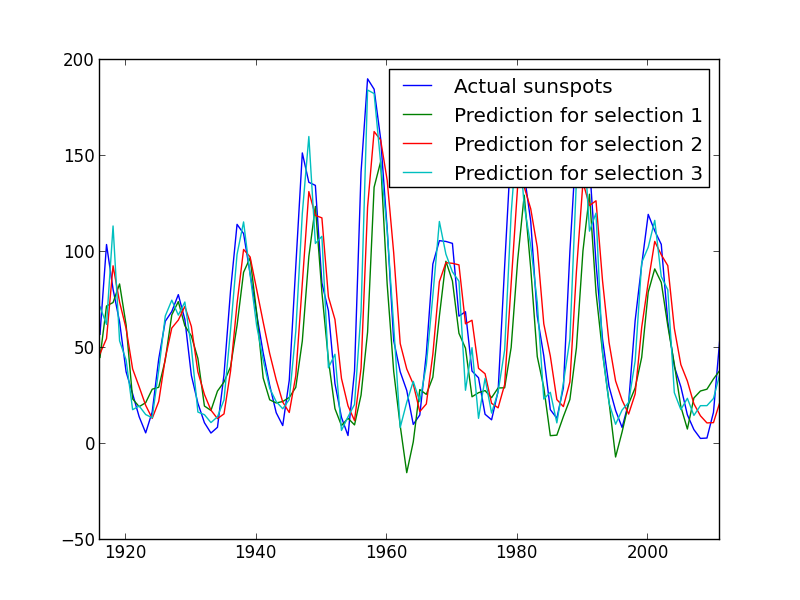
\includegraphics[width=1.0\textwidth]{figures/figure_II_2_1_2}
      \caption{Years versus predicted sunspots for each model along with the actual sun spot number.}
      \label{fig:years_vs_predicted}
    \end{figure}

  \subsection*{II.2.2 Maximum a posteriori solution}

    Figures \ref{fig:map_estimate_alpha1}, \ref{fig:map_estimate_alpha2} and \ref{fig:map_estimate_alpha3} show the results for different values of $\alpha$ using our obtained MAP estimates. Figures \ref{fig:map_estimate_alpha1} and \ref{fig:map_estimate_alpha2} show that for the selection model 1 and 2 the error increases when increasing $\alpha$, but for the third one the error sharply decreases until $\alpha$ reaches 20 and then steadily increases up to 18.68 for $\alpha = 100$, which is still lower than the initial error for $\alpha = 0$.
    \begin{figure}[h]
      \centering
        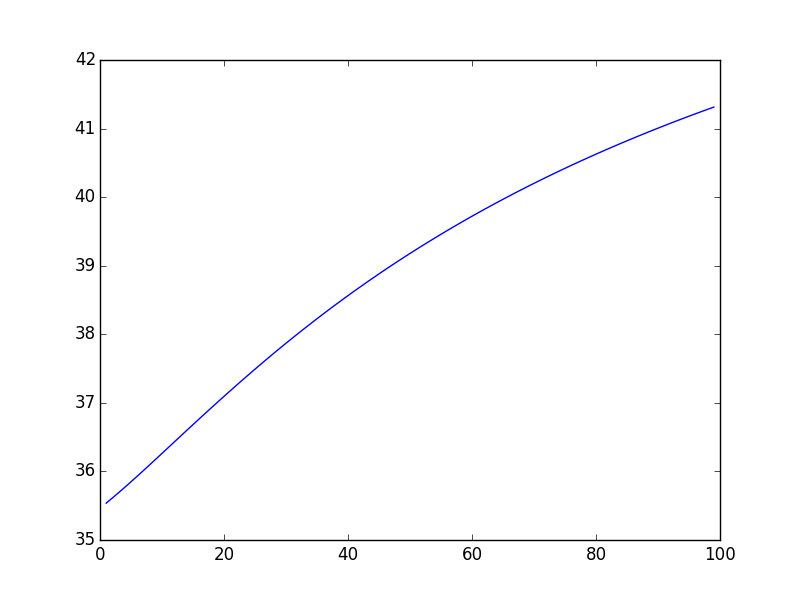
\includegraphics[width=0.8\textwidth]{figures/figure_II_2_2_1}
      \caption{MAP estimates for \textbf{selection 1} using different $\alpha$}
      \label{fig:map_estimate_alpha1}
    \end{figure}
    \begin{figure}[h]
      \centering
        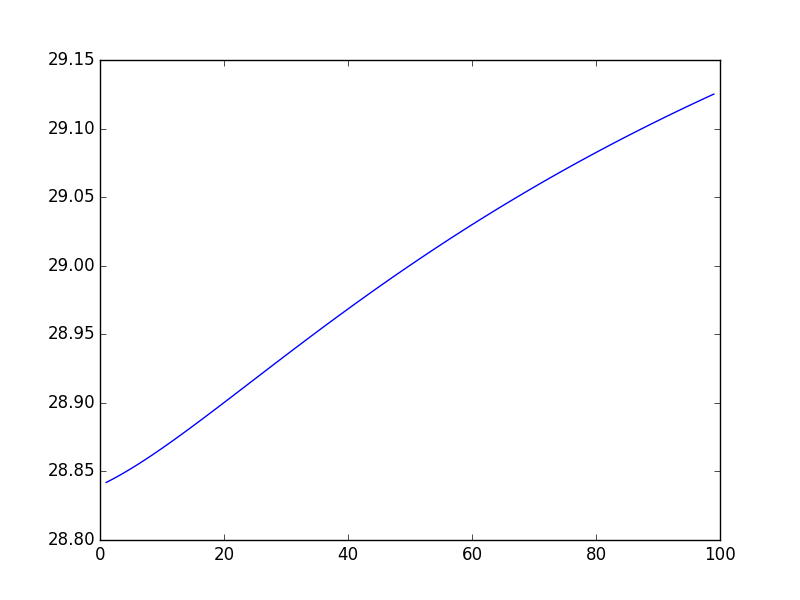
\includegraphics[width=0.8\textwidth]{figures/figure_II_2_2_2}
      \caption{MAP estimates for \textbf{selection 2} using different $\alpha$}
      \label{fig:map_estimate_alpha2}
    \end{figure}
    \begin{figure}[h]
      \centering
        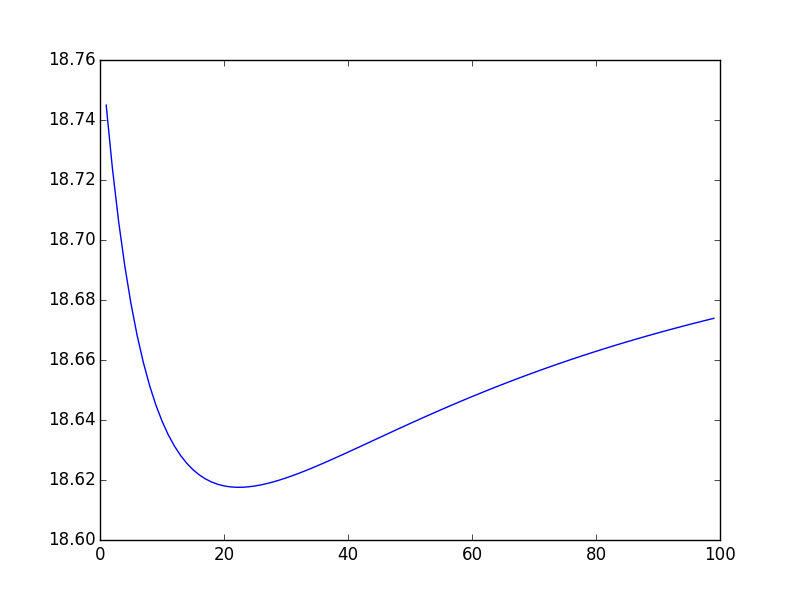
\includegraphics[width=0.8\textwidth]{figures/figure_II_2_2_3}
      \caption{MAP estimates for \textbf{selection 3} using different $\alpha$}
      \label{fig:map_estimate_alpha3}
    \end{figure}

  \subsection*{II.2.3 Weighted sum-of-squares (based on CB Ex. 3.3)}
  
    Start by calculating $\bigtriangledown E_D(w)$

    \begin{align*}
      \bigtriangledown E_D(w) &= \frac{1}{2} \sum\limits_{n=1}^N r_n\bigtriangledown_w (t_n - w^T\phi(x_n))^2 \\
                              &= \frac{1}{2} \sum\limits_{n=1}^N r_n * 2 [t_n - w^T\phi(x_n)] \bigtriangledown_w (t_n - w^T\phi(x_n)) \\
                              &= \sum\limits_{n=1}^N r_n [t_n - w^T\phi(x_n)]\phi(x_n^T) \\
    \end{align*}
    and find where $\bigtriangledown_wE_D(w)$ equals zero:

    \begin{align*}
      \sum\limits_{n=1}^N r_n [t_n - w^T\phi(x_n)]\phi(x_n^T) &= 0 \\
      [\sum\limits_{n=1}^N r_nt_n\phi(x_n)^T] - w^T[\sum\limits_{n=1}^N r_n\phi(x_n)\phi(x_n)^T] &= 0 \\
      [\sum\limits_{n=1}^N r_nt_n\phi(x_n)^T] &= w^T[\sum\limits_{n=1}^N r_n\phi(x_n)\phi(x_n)^T] \\
      w^T &= [\sum\limits_{n=1}^N r_nt_n\phi(x_n)^T][\sum\limits_{n=1}^N r_n\phi(x_n)\phi(x_n)^T]^{-1}
    \end{align*}
    Comparing given equation with equation 3.11 and 3.13 on page 141 of Bishop, we can say that $r_{n}$ can be regarded as an inverse variance factor specific to the data point $(x_{n}, t_{n})$ that can be interpreted as a scaling (or even replacing) of $\beta$.

    The interpretation that we found out is that $r_{n}$ can represent an effective number of replicated observations of the specific instance $(x_{n}, t_{n})$, particularly if we restrict $r_{n} \epsilon$  Z+. 


\end{document}
% End of document.







